%%%% ijcai25.tex

\typeout{IJCAI--25 Instructions for Authors}

% These are the instructions for authors for IJCAI-25.

\documentclass{article}
\pdfpagewidth=8.5in
\pdfpageheight=11in

\usepackage{ijcai25}

% Use the postscript times font!
\usepackage{times}
\usepackage{soul}
\usepackage{url}
\usepackage[hidelinks]{hyperref}
\usepackage[utf8]{inputenc}
\usepackage[small]{caption}
\usepackage{graphicx}
\usepackage{amsmath}
\usepackage{amsthm}
\usepackage{booktabs}
\usepackage{algorithm}
\usepackage{algorithmic}
\usepackage[switch]{lineno}

% Comment out this line in the camera-ready submission
\linenumbers

\urlstyle{same}

\usepackage{pifont} % 引入 pifont 宏包
\usepackage{amssymb} % 引入 amssymb 宏包
\usepackage{graphicx} % For including images
\usepackage{booktabs} % For three-line tables
\usepackage{tabularx} % For adjustable table width
\usepackage{array}
\usepackage{makecell} % 用于单元格内容换行和居中

% Use the postscript times font!
\usepackage{times}
\usepackage{soul}
\usepackage{url}
\usepackage[hidelinks]{hyperref}
\usepackage[utf8]{inputenc}
\usepackage[small]{caption}
\usepackage{graphicx}
\usepackage{booktabs}
\usepackage{algorithm}
\usepackage{algorithmic}
\usepackage[switch]{lineno}
\usepackage{algorithm}
\usepackage{algorithmic}
\usepackage{amsfonts}
\usepackage{amsthm,amsmath,amssymb}
\usepackage{mathrsfs}
\usepackage{booktabs}
\usepackage{graphicx}
\usepackage{subfig}
\newtheorem{theorem}{Theorem}
\usepackage{color}
\usepackage{graphicx} % 用于插入图片
\usepackage{array}    % 用于调整表格格式
\usepackage{multirow} % 用于合并单元格
%% 自定义代码块的风格
\documentclass{article}
\usepackage{listings} % 引入 listings 宏包
\usepackage{xcolor}   % 引入颜色支持

% 定义 JSON 格式的高亮样式
\lstdefinestyle{json}{
    basicstyle=\ttfamily\footnotesize,
    commentstyle=\color{gray},
    stringstyle=\color{red},
    keywordstyle=\color{blue},
    numbers=left,
    numberstyle=\tiny\color{gray},
    breaklines=true,
    frame=single,
    captionpos=b,
    showstringspaces=false
}\definecolor{codegreen}{rgb}{0,0.6,0.1}
\definecolor{codegray}{rgb}{0.5,0.5,0.5}
\definecolor{codepurple}{rgb}{0.58,0,0.82}
\definecolor{backcolour}{rgb}{0.95,0.95,0.92}
\lstdefinestyle{mystyle}{
    backgroundcolor=\color{backcolour},   
    commentstyle=\color{codegreen},
    keywordstyle=\color{magenta},
    numberstyle=\tiny\color{codegray},
    stringstyle=\color{codepurple},
    basicstyle=\ttfamily\footnotesize,
    breakatwhitespace=false,         
    breaklines=true,                 
    captionpos=b,                    
    keepspaces=true,                 
    numbers=left,                    
    numbersep=4pt,         % 行号和代码的距离          
    showspaces=false,                
    showstringspaces=false,
    showtabs=false,                  
    tabsize=2
}

\lstset{style=mystyle}

\usepackage[utf8]{inputenc}


\pdfinfo{
/TemplateVersion (IJCAI.2024.0)
}

\title{\textit{ComplexOvercooked}: A Dynamic-Objective Challenge for Cooperative Multi-Agent Reinforcement Learning}


% Single author syntax
\author{
    Author Name
    \affiliations
    Affiliation
    \emails
    email@example.com
}

% Multiple author syntax (remove the single-author syntax above and the \iffalse ... \fi here)
\iffalse
\author{
First Author$^1$
\and
Second Author$^2$\and
Third Author$^{2,3}$\And
Fourth Author$^4$
\affiliations
$^1$First Affiliation\\
$^2$Second Affiliation\\
$^3$Third Affiliation\\
$^4$Fourth Affiliation
\emails
\{first, second\}@example.com,
third@other.example.com,
fourth@example.com
}
\fi

\begin{document}

\maketitle
\begin{abstract}
% Overcooked is a classic multi-agent cooperative game scenario. Existing simulation environments utilize simplified game settings to achieve cooperation between agents as well as human-agent collaboration tasks. However, these environments lack key features present in the real Overcooked game, such as ingredient synthesis, four-player cooperation and the most important, dynamic objectives. As a result, in Overcooked, a bounded-reward environment, the performance of agents has little improvement margin, which is detrimental to research in multi-agent reinforcement learning. 
Recent advancements in cooperative multi-agent systems have led to significant updates in both environments and algorithms. However, current cooperative multi-agent reinforcement learning (MARL) environments predominantly focus on single-objective tasks, where agents optimize their policies toward single static objectives. For instance, in the \textit{Overcooked\_AI} environment, agents are tasked with delivering as many orders as possible within a limited time, without considering the actual demand or necessity of these orders by users. This contrasts sharply with the real-world Overcooked game scenario, where the primary challenge lies in fulfilling dynamic user orders promptly. To address this gap, we introduce \textit{ComplexOvercooked}, a novel MARL environment designed to better simulate real-world complexities. This environment features a highly configurable layout, dynamically generated user order demands, and supports three distinct control interfaces: human, model-based Large Language Models (LLM), and model-free Reinforcement Learning (RL) agents. By benchmarking classic MARL algorithms in \textit{ComplexOvercooked}, we not only highlight the potential for performance enhancement but also delineate the capability boundaries of MARL within this more intricate setting. We public the code of environment and MARL algorithms at https://anonymous.4open.science/r/ComplexOvercooked-1D82.
\end{abstract}

\section{Introduction}
\label{sec:intro}
% 1. 多智能体合作任务中常常关注部分可观测,非平稳性和信用分配等问题,而动态目标问题同样重要,例如,在经典的分手厨房游戏中,智能体完成的订单需要匹配用户的需求,同样的订单在分别在时间步1和时间步2送出,可能得到是奖励和惩罚。当前的合作MARL环境中尚未考虑动态目标的问题,流行的overcookedAI也是如此。
% 2. 动态任务目标问题很难,因为在MARL问题中加入了优化目标的随机性,优化目标改变时,智能体已经学到的策略却无法得到既定奖励,甚至得到惩罚,这会导致策略梯度朝着与目标改变之前相反的方向更新网络的权重,但是这个问题从直觉上而言是MARL可以解决的,因为在完全可观测的博弈环境中,目标变化时环境的state发生改变,这对智能体是已知的。
% 3. ComplexOvercooked和overcooked\_ai的对比, 列表,并简单介绍我们的环境
% 4. 我们的贡献可以总结如下:
% 1. 我们提出了一个多智能体强化学习的环境, ComplexOvercooked,这个环境还原了真实游戏的配置,对用户很友好并且易于配置,有利于拓展合作智能体的能力边界。
% 2.我们在ComplexOvercooked配置了键盘、智能体,和LLM的控制接口,可以轻易地收集人类玩家的数据,便于人机合作算法以及合作大模型算法的研究。
% 3. 我们在多个自定义的ComplexOvercooked布局中测试了经典MARL算法的性能,证实了在该环境中增强MARL算法性能的潜力。
In multi-agent cooperative tasks, significant attention is often given to issues such as partial observability\cite{zhu2022survey}, non-stationarity\cite{papoudakis2019dealing}, and credit assignment \cite{wang2021towards}. However, the challenge of dynamic objectives is equally important. For example, in the classic Overcooked game, the orders completed by agents must match user demands. The same order, if delivered at timestep $t_1$ versus timestep $t_2$, may result in either a reward or a penalty. Current cooperative MARL environments, including the popular \textit{Overcooked-AI} \cite{carroll2019utility}, have yet to address the challenge of dynamic objectives.

The problem of dynamic objectives is challenging because it introduces randomness into the optimization goals of MARL. When the optimization goal changes, the policies learned by the agents may no longer yield the expected rewards and could even result in penalties. This can cause the policy gradient to update the network weights in a direction opposite to that before the goal change. However, intuitively, this problem is solvable within the MARL framework since the state of the environment changes as the goal changes, and this information can be observed by agents.
\begin{table}[!t]
\centering

\caption{Comparison of Overcooked RL environments}
\label{tab:overcooked_comparison}
\begin{tabularx}{\linewidth}{>{\centering\arraybackslash}X >{\centering\arraybackslash}X >{\centering\arraybackslash}X}

\toprule
\textbf{} & \textbf{Overcooked\_AI} & \textbf{ComplexOvercooked} \\
\midrule
\textbf{\makecell[c]{Game interface\\\\\\\\\\}} & 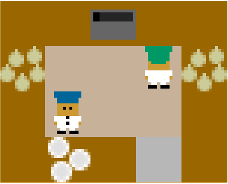
\includegraphics[width=2.8cm]{Figures/overcooked_ai.png} & 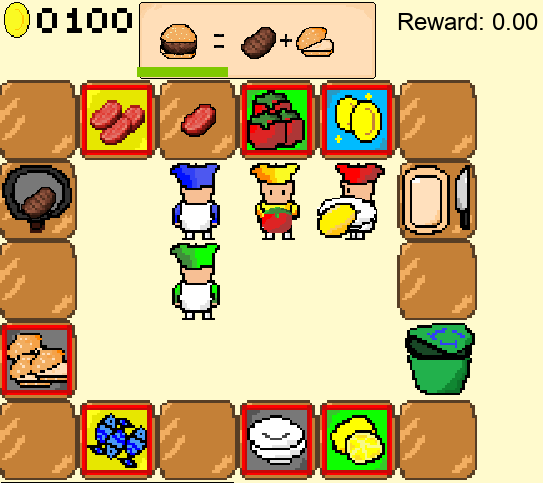
\includegraphics[width=2.8cm]{Figures/complexOvercooked_interface.png} \\[-20pt]
\textbf{4 players} & \ding{55} & \ding{51} \\
\textbf{Dynamic orders} & \ding{55} & \ding{51} \\
\textbf{Synthesis} & \ding{55} & \ding{51} \\
\textbf{LLM control} & \ding{55} & \ding{51} \\
\textbf{\# of interactable objects} & \makecell[c]{\\6} & \makecell[c]{\\18} \\
\bottomrule
\end{tabularx}
\end{table}


In this paper, we introduce \textit{ComplexOvercooked}, a MARL environment that highly replicates the mechanics of the real Overcooked game. Using this environment, dynamic task objectives such as order types, quantities, and durations can be easily configured. Compared to the popular \textit{Overcooked-AI}, \textit{ComplexOvercooked} features more complex game logic (e.g., diverse order synthesis paths), a wider variety of interactive objects, and supports cooperative training for up to four agents (Table \ref{tab:overcooked_comparison}). To demonstrate the potential of this environment in human-agent collaboration tasks, we have integrated control interfaces for both humans and LLMs, enabling easy data collection and the use of LLMs to enhance agent capabilities. We benchmarked the environment using classical MARL algorithms, demonstrating that the environment offers expandable capability boundaries for MARL algorithms. Our contributions can be summarized as follows:
\begin{enumerate}
\item We propose a novel dynamic-objective MARL environment, \textit{ComplexOvercooked}, which faithfully replicates the configurations of the Overcooked game. It is user-friendly, highly configurable, and designed to push the boundaries of cooperative agent capabilities.
\item We integrate multiple control interfaces in \textit{ComplexOvercooked}, including keyboard, model-free RL agent, and model-based LLM controls. This enables seamless collection of human player data, facilitating research on human-agent collaboration algorithms and cooperative LLM algorithms.
\item We benchmark the performance of classical MARL algorithms in various custom layouts of \textit{ComplexOvercooked}. Our experiments demonstrate the potential for enhancing MARL algorithm performance in this environment, highlighting its value as a benchmark for future research.
\end{enumerate}

% Training collaborative agents is a highly popular direction in the field of artificial intelligence. A capable collaborative agent can enhance collaborative performance, influence human behavior \cite{hong2023learning}, and achieve alignment with human values \cite{yuan2022situ} when working alongside humans to accomplish complex tasks. Currently, the training of collaborative agents based on deep reinforcement learning (DRL) primarily relies on the following environments: \textit{Overcooked} \cite{carroll2019utility}, Hanabi \cite{bard2020hanabi}, Multi-Agent Particle Environment (MPE) \cite{lowe2017multi}, Google Research Football (GRF) \cite{kurach2020google} and Starcraft Multi-Agent Challenge(SMAC) \cite{vinyals2017starcraft,samvelyan2019starcraft}. 

% Previous studies are based on the original \textit{Overcooked} game, and these works mainly include the following aspects: zero-short coordination (ZSC) \cite{yu2023learning,zhao2023maximum,strouse2021collaborating,li2023cooperative}, human-AI collaboration \cite{carroll2019utility,strouse2021collaborating,hong2023learning}, robustness analysis of collaborative agents\cite{knott2021evaluating}, and the application of large language models (LLM) in Collaboration \cite{wen2022multi,zhang2023proagent,guan2023efficient,zhu2023madiff}. Although these studies propose algorithms that perform well in original \textit{Overcooked}, they make the improvement margin small\cite{yu2023learning}, which is disadvantageous for the development of collaborative agents.

% The original \textit{Overcooked} environment limits the training of collaborative agents for the following main reasons: Firstly, the game logic is simplified compared to the real \textit{Overcooked} game. \textit{Overcooked} is actually a multiplayer, multitask cooperative game, with up to four players. In it, agents may need to finish multiple orders simultaneously, and multiple agents must have a sense of division of labor and task allocation when completing tasks. These capabilities are not sufficiently reflected in the original \textit{Overcooked} environment. In many \textit{Overcooked} game layouts, one player can do the work of two, and the presence of a companion can actually interfere with an individual agent's actions and path planning. Furthermore, the tasks in \textit{Overcooked} are relatively simple. For example, to make onion soup, one just needs to put three onions in a pot, cook, and serve it to serving area. This results in a rather monotonous workflow of cooperation between agents, where typically one agent places raw onions in the pot while another delivers the soup with a plate. More diverse workflow of cooperation would better test the coordination and collaboration between agents and are beneficial for training agents with superior cooperative abilities.

% 我们提出一个新颖的多人协同的,多任务的overcook\_pygame环境,这个环境更接近真实的overcook游戏。如下图1中所示,智能体需要在规定时间内完成多个特定任务,每道菜的合成路径在上方的任务栏中显示,例如:完成一个番茄牛肉汉堡的过程可能是:将番茄切好,将牛肉放在平底锅中煮熟,在用汉堡和切好的番茄以及煮熟的牛肉合成最终的番茄牛肉汉堡。此外,本环境引入了垃圾回收机制,因为可能有些菜可能未再规定时间内完成,可将其倒入垃圾桶,从而不占桌面空间。总的来说,和之前被广泛使用的合作环境相比,overcook_pygame带来了以下挑战:首先,overcook_pygame是多任务的,同一时间有多个任务需要完成,这有利于研究智能体的信度分配和行为偏好,其次是任务流程复杂多样,完成特定任务的方式可能有多种。overcook_pygame具有高度的可塑性 scalability,玩家可以轻易的修改地图元素,智能体数量和任务类别,任务时间等。此外,我们还提供了大模型的接口便于AI-AI或者人与AI的通讯以实现更好的合作效能。

% We propose a novel multiplayer, multitasking \textit{Overcooked pygame} environment that closely resembles the real \textit{Overcooked} game. As shown in Figure \ref{fig:intro}, agents must complete multiple specific tasks within a limit time. The synthesis steps for each order is displayed in the task menu above. For example, the process of making a \textit{ACtoamtocookedbeefhamburger} might involve chopping tomatoes, cooking beef in a frying pan, and then combining the burger with chopped tomatoes and cooked beef to make the final \textit{ACtoamtocookedbeefhamburger}. Additionally, our environment introduces a garbage recycling mechanism, as some dishes may not be completed within the allotted time and can be dumped into the trash, thereby not occupying table space. Overall, compared to other cooperative environments, \textit{Overcooked pygame} presents the following challenges: Firstly, \textit{Overcooked pygame} is multi-tasking, with multiple tasks to be completed simultaneously, which facilitates research on agent's trust allocation and behavior preferences. Secondly, the task flows are complex and diverse, with multiple possible ways to complete specific tasks. \textit{Overcooked pygame} possesses a high degree of scalability and provides interfaces for large language models (LLM) to facilitate AI-AI or human-AI communication for an improved collaborative performance.



\section{Related Work}
\label{sec:related}
\subsection{Environments of cooperative MARL}
In the field of reinforcement learning, the design and study of cooperative environments are crucial for the development of multi-agent systems. Cooperative reinforcement learning environments typically involve multiple agents working together to achieve a common goal, requiring collaboration among agents. Some popular environments such as Multi-Agent Particle Environment (MPE)\cite{lowe2017multi}, StarCraft II \cite{vinyals2017starcraft}, GRF\cite{kurach2020google} and Hanabi\cite{bard2020hanabi} are widely used and typically feature single and well-defined objectives, which remain unchanged despite the randomness of state transitions. 

In contrast, our proposed ComplexOvercooked is a multi-objective simulation environment where task objectives (orders) are dynamically updated. This introduces additional non-stationarity into the learning process of MARL agents. Furthermore, Overcooked is inherently a communication-based game, where players collaborate through natural language during gameplay. ComplexOvercooked fully considers this aspect and, in addition to human and RL agent controls, provides an interface for LLM control. This facilitates future research on LLM-enhanced reinforcement learning.
% 现有的合作任务仿真环境的任务目标单一且明确,且不会因为环境状态转移的随机性而改变。我们提出的ComplexOvercooled是一个多目标的仿真环境,任务目标(订单)会随机更新,这为MARL智能体的学习引入了更多非平稳性,此外,Overcooked本身是一款交流游戏,在合作的过程中,玩家之间通过自然语言进行交流,ComplexOvercooled充分考虑了这一事实,除了人和RL智能体,开发了大模型控制的接口,这有助于大模型增强的强化学习未来研究。
\subsection{Cooperative multi-agent reinforcement learning}
Although cooperative Multi-Agent Reinforcement Learning (MARL) has emerged as a powerful framework for addressing large-scale, complex, real-time, and uncertain problems in cooperative scenarios, it also introduces several challenges that need to be addressed. First, in partially observable environments, agents can only access local information, making it difficult for them to make optimal decisions independently\cite{zhu2022survey}. Second, the simultaneous learning of multiple agents results in a non-stationary environment, complicating policy convergence \cite{papoudakis2019dealing}. Third, cooperative MAS often relies on shared rewards, raising the challenge of credit assignment—how to allocate rewards effectively to guide individual agents toward cooperative behavior and maximize system performance \cite{wang2021towards}. Finally, as the number of agents increases, the search space for policy learning grows exponentially, posing scalability issues and making policy optimization increasingly difficult \cite{zhang2011scaling,christianos2021scaling}.

To tackle these challenges, researchers have developed a variety of algorithms to enhance agent cooperation, including policy gradient-based methods like MADDPG \cite{lowe2017multi} and MAPPO \cite{yu2022surprising}, value-based methods such as VDN \cite{sunehag2017value} and QMIX \cite{rashid2020monotonic}, and Transformer-based approaches like MAT \cite{wen2022multi}, which leverage advanced architectures to improve coordination. These methods have achieved remarkable success in benchmark environments shown in the Section 2.1. 
% 尽管协作多智能体强化学习(MARL)已成为解决协作场景中大规模、复杂、实时和不确定问题的强大框架,但它也带来了一些需要解决的挑战。首先,在部分可观测环境中,智能体只能获取局部信息,这使得它们难以独立做出最优决策[20]。其次,多个智能体同时学习导致环境非平稳,增加了策略收敛的难度[21]。第三,协作式MAS通常依赖于共享奖励,这引发了信用分配问题——如何有效分配奖励以引导个体智能体实现协作并最大化系统性能[22]。最后,随着智能体数量的增加,策略学习的搜索空间呈指数级增长,带来了可扩展性问题,使得策略优化变得愈发困难[23, 24]。
\subsection{Human-AI collaboration}
Much recent work has focused on designing collaborative agents towards humans in the original \textit{Overcooked\_AI} environment. Behavioral cloning play (BCP) \cite{carroll2019utility} is the first proposed algorithm for human-AI collaboration in \textit{Overcooked}, which relies on human experts' data. Fictitious Co-Play (FCP) \cite{strouse2021collaborating} is a zero-shot coordination (ZSC) (also known as ad-hoc team-play \cite{stone2010ad}) algorithm that mainly consists of two stages. In the first stage, it trains a population of self-play agents and save their ``checkpoint'' representing their strategy at that point in time. In the second stage, it trains the FCP agent by teaming up it with various ``checkpoints''. While training FCP agent is somewhat time-consuming and resource-intensive, it performs well when it collaborates with unseen humans. Subsequent works following FCP have augmented the policy pool for a stronger adaptive policy by using biased strategy \cite{yu2023learning} or population entropy bonus \cite{zhao2023maximum}. Some other algorithms also focus on exploring the edge cases of collaborative agents \cite{knott2021evaluating}, modeling systematic suboptimality of humans \cite{laidlaw2022boltzmann} and reusing optimal policy via Bayesian policy reuse \cite{wangbeyond} to improve the human's performance in collaborative tasks. 
% \subsection{Multi-agent task allocation}
% Task allocation has been extensively studied in the field of multi-agent systems\cite{gerkey2004formal,khamis2015multi}. In this context, the primary objective is to effectively assign agents to tasks from a given set, with the aim of maximizing overall utility. It is assumed that a utility function, which associates utility values with agent team-task pairs, is provided for this purpose. This allocation process plays a crucial role in optimizing the overall performance and efficiency of multi-agent systems and robotic operations.
% According to taxonomy of task allocation in multi-agent systems \cite{gerkey2004formal}, \textit{Overcooked pygame} problem can be classified into ST-MR-IA (single-task agents, multi-agent tasks, instantaneous allocation). That is, multiple tasks need to be executed simultaneously, and the same task requires collaboration among multiple agents to complete. Recently, some works focus on allocating agents to different subtasks. However, these subtasks offen have a fixed workflow \cite{iqbal2022alma} or lack semantic meanings as a latent variable \cite{yang2022ldsa}. \textit{Overcooked pygame} is an environment where multiple tasks should be executed synchronously, and the workflow of each subtask varies due to the behavioral preferences of agents, posing a challenge in the field of task allocation.

\section{Preliminaries}
\label{sec:preliminary}
\subsection{Cooperative multi-agent MDP}
\textit{ComplexOvercooked} is a fully cooperative and fully observable MARL environment. The multi-agent Markov decision process (MDP) can be modelled by a tuple $\langle S,a,\{A_{i\in{a}}\},\mathcal{T},\mathcal{R},d^0 \rangle$ with a finite set of states $\mathcal{S}$, a real-value reward function $\mathcal{R}:\mathcal{S}\times \mathcal{A} \to \Delta(\mathbb{R}) $. $a$ is a finite set of agents; $A\_{i}$ is the finite set of actions available to agent $i$, $d^0$ is the start-state distribution. 
A transition function $\mathcal{T}:S\times A_{1}\times\cdots\times A_{n} \to \Delta(\mathcal{S})$ specifies the distribution over next states, where $\Delta$ denotes a conditional distribution.

\subsection{Original \textit{Overcooked\_AI} environment}
The original \textit{Overcooked\_AI} environment is introduced in \cite{carroll2019utility}. In this game, two players should cooperate to finish as many orders as possible within a limited time. The steps to complete a dish are: putting three onions in a pot, taking the cooked onion out of the pot with a plate, and delivering the plate with onion soup to the serving area. The players can move to face any objects and interact with them. The action space of the environment is a set of $\{up, down, left, right, stay, interact\}$. The observation space is defined by a vector which consider each player’s facing direction, absolute position and relative positions to: the partner, the closest onion, the closest pot, the closest dish, the closest serving area, etc.




\section{\textit{ComplexOvercooked} Environment}
\label{sec:cbpr}
\textit{ComplexOvercooked} is an open-source RL environment for all researchers for any non-commercial activity under the MIT License. In this section, we will introduce dynamic-objective challenges in this environment, order synthesis paths, and core elements (i.e., observation space, action space, and reward function setups) of RL agents. We provide three types of interfaces supporting RL agents, humans and LLMs. We emphasize the differences in these settings compared to that in original \textit{Overooked\_AI}.
\begin{figure}[htb]
    \centering
    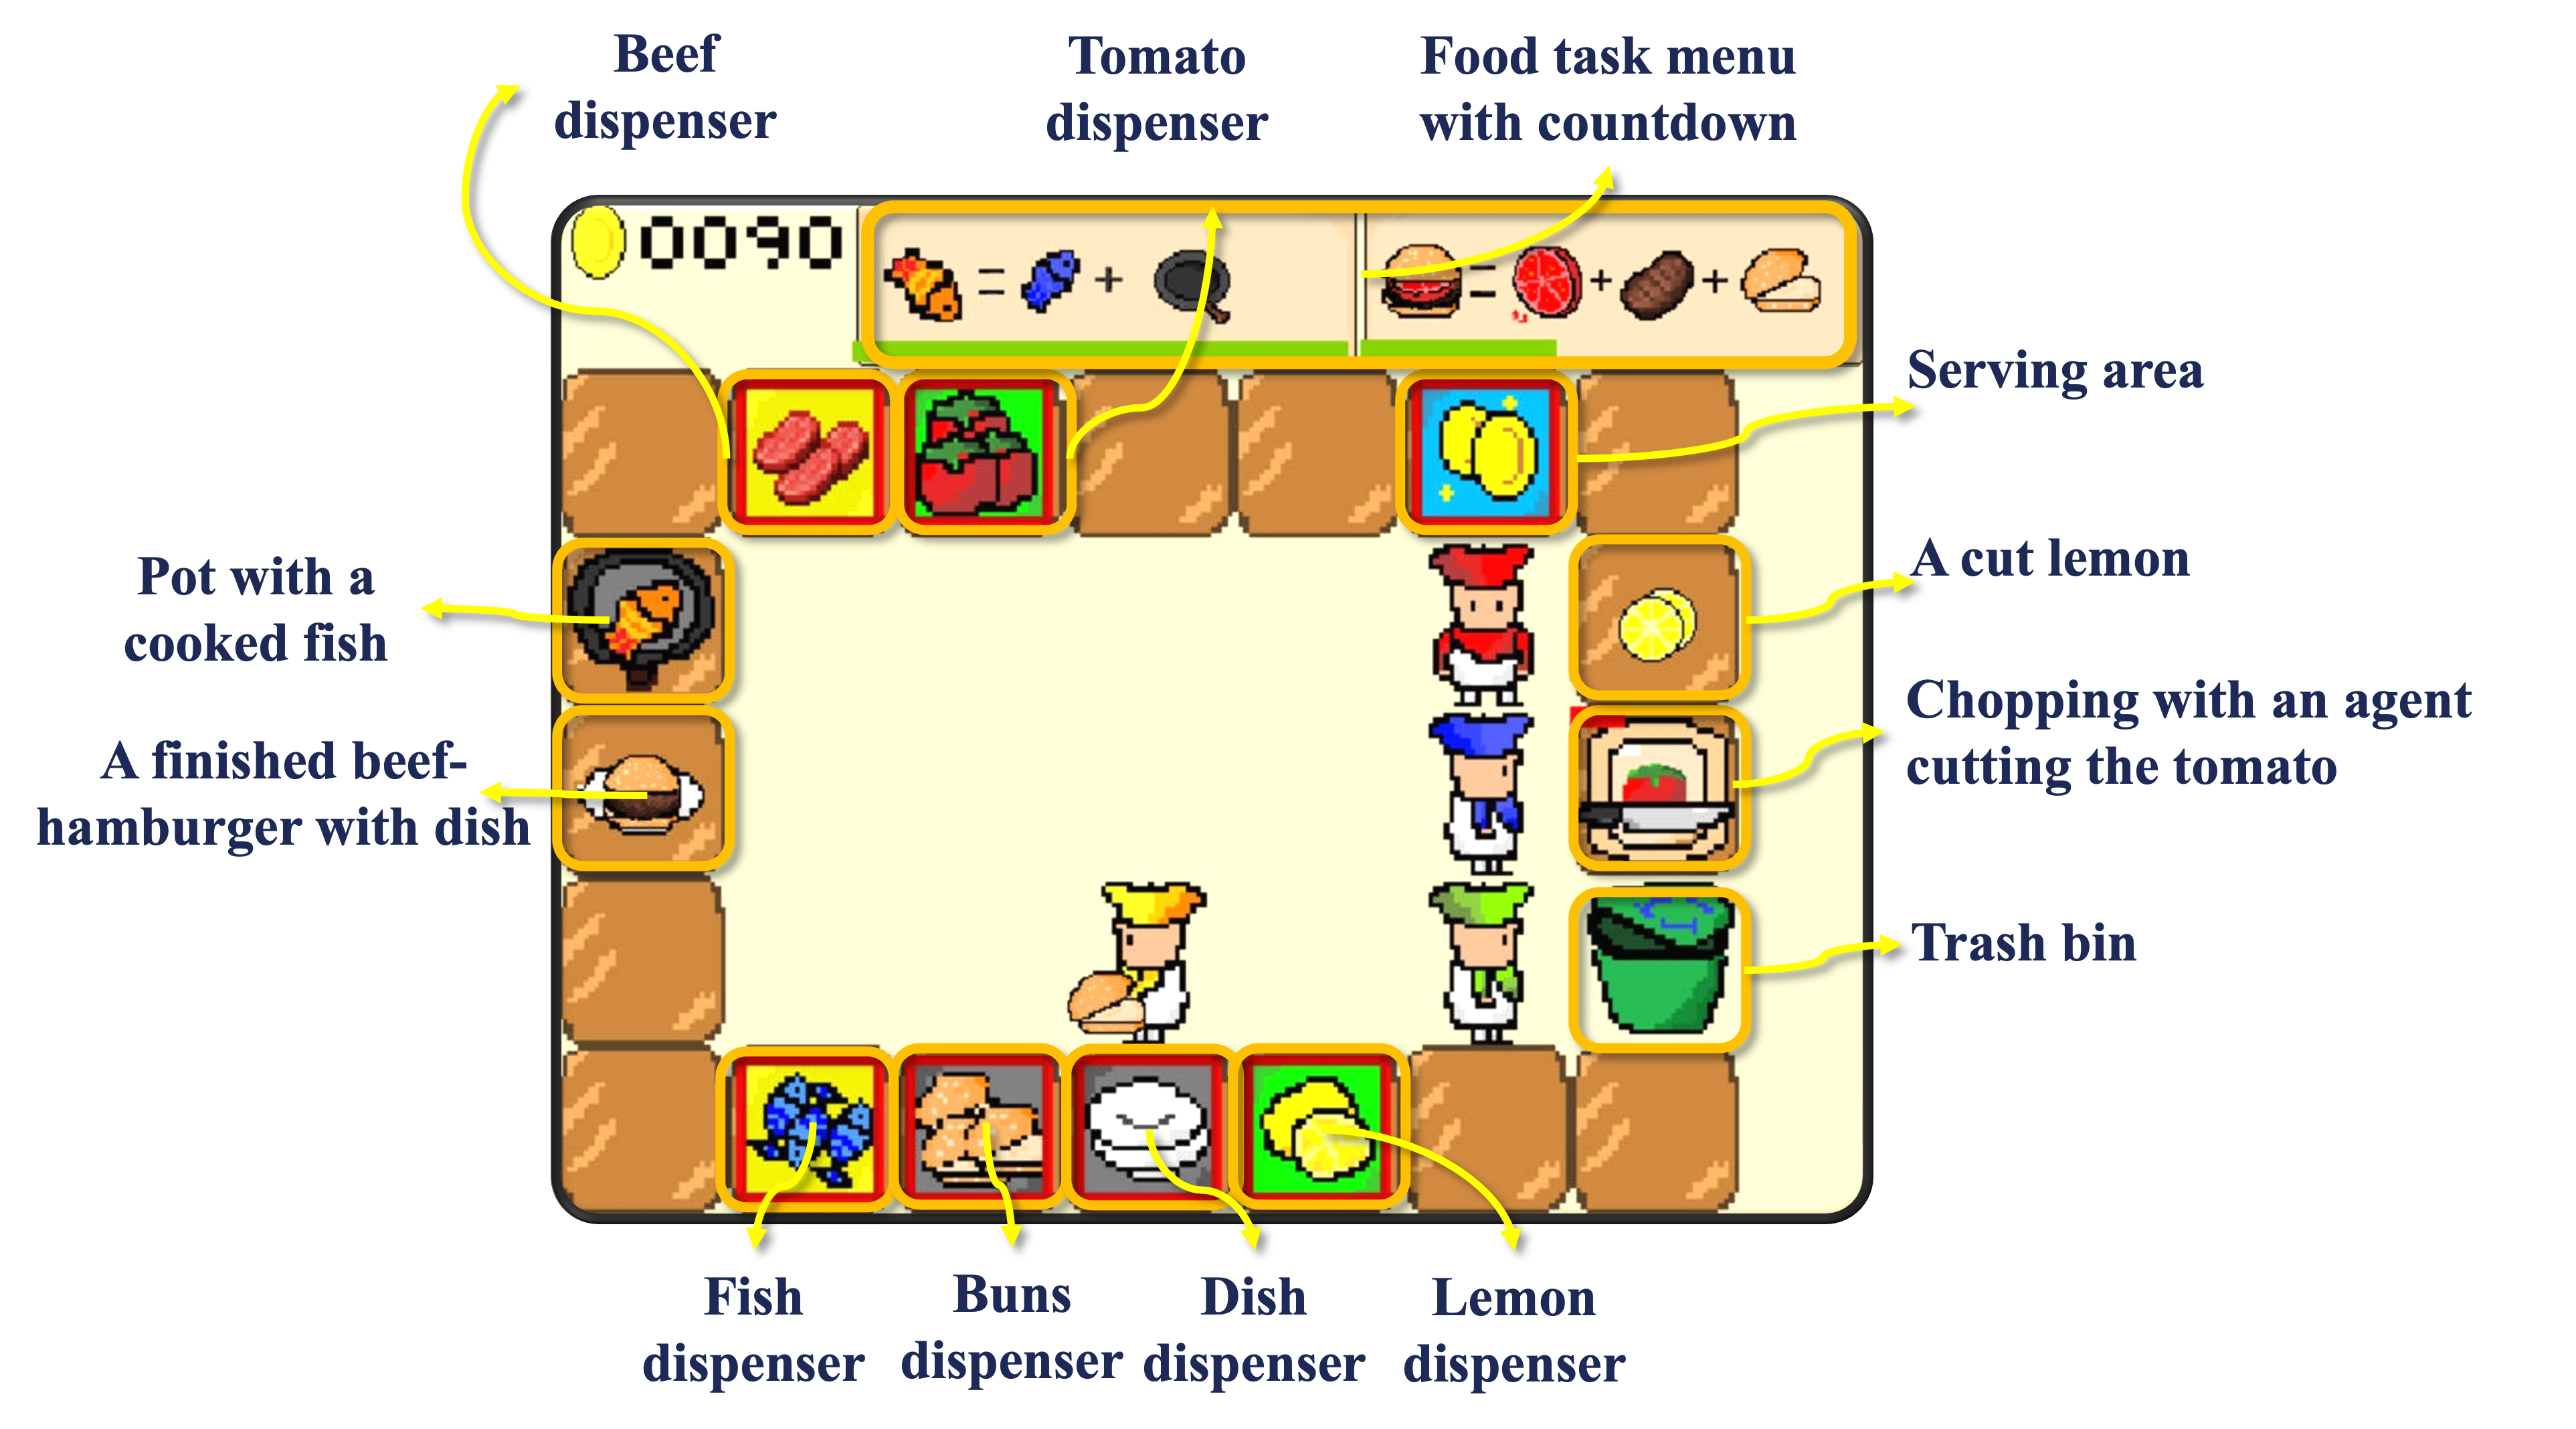
\includegraphics[width=\linewidth]{Figures/game_intro.png}
  \caption{The game interface of \textit{ComplexOvercooked}, in which multiple orders are generated randomly and they need to be finished simultaneously as listed in the task menu.}
\label{fig:intro}
\end{figure}
\subsection{Dynamic-objective challenge}
In the Overcooked game, players need to cook specific dishes based on user orders (shown at the top of Figure \ref{fig:intro}). Different orders are randomly generated and have distinct synthesis paths (Figure \ref{fig:recipe}), which determine whether the user's current actions will receive rewards. In the default game configuration, each order lasts for 200 time steps, and users must complete the cooking within this time frame. Failing to deliver the order within the time limit results in no reward or even a penalty. This dynamic objective poses a significant challenge for multi-agent training.

In the current game, we provide four types of orders: \textit{Cookedfish}, \textit{Cookedbeefhamburger}, \textit{AClemoncookedfish} and \textit{ACtomatocookedbeefhambuger}. These orders vary in difficulty and reward. For example, the steps required for \textit{AClemoncookedfish} are: cook fish using a pot, cut lemon using a cutting table and combine the cooked fish and cut lemon,  while \textit{Cookedfish} is much simpler, requiring only placing raw fish into the pot, waiting for a certain time, and then serving it on a plate. Higher-difficulty orders take more time to complete but yield greater rewards, forcing agents to make trade-offs during training.
\begin{figure}[H]
    \centering
    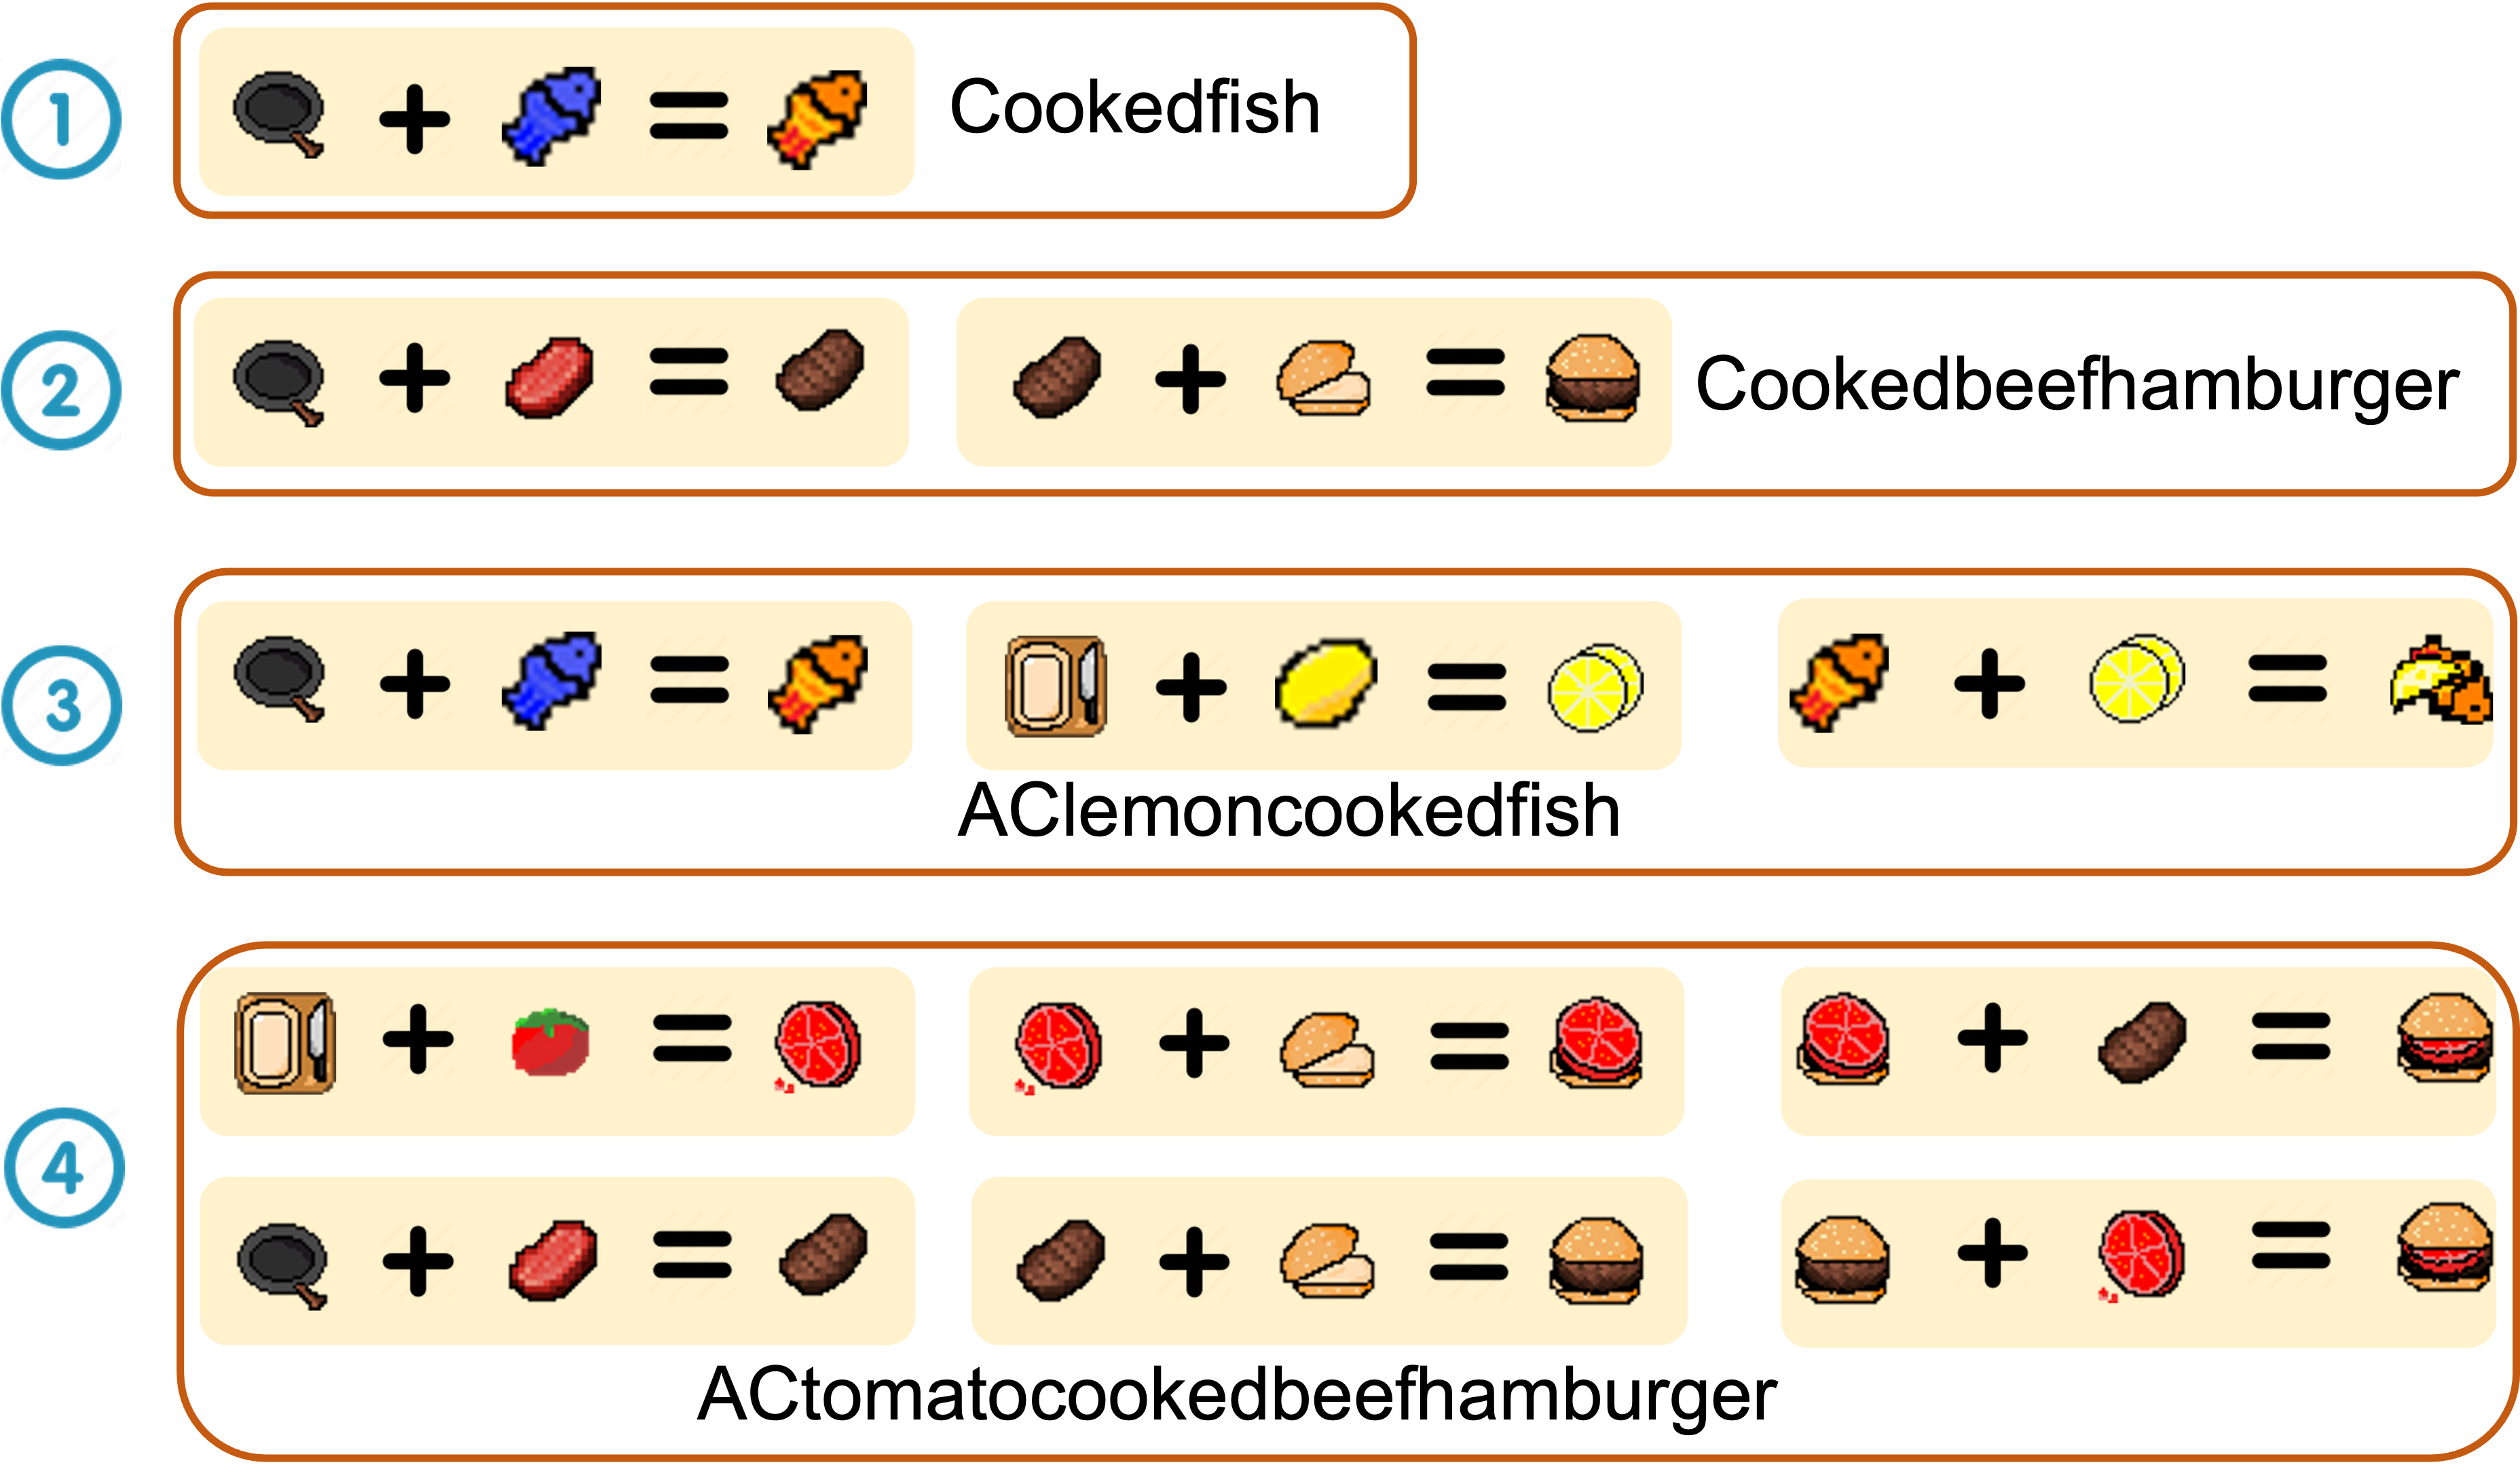
\includegraphics[width=\linewidth]{Figures/recipe.png}
  \caption{Recipes and synthesis paths of orders in \textit{ComplexOvercooked}}
\label{fig:recipe}
\end{figure}

\subsection{Control interfaces}
To empower research in the field of collaboration among agents, LLMs, and humans, we provide three types of control interfaces to facilitate the study of subsequent control algorithms.\\
\textbf{Human} \ Human players can control the actions of the chef in the game via the keyboard and can set one of the chefs as an AI to conduct a human-AI cooperation. In addition, the trajectories of human players can be easily collected for imitation learning. \\
\textbf{RL agent} \ Based on observations of the environment, RL agent can decide on a sequence of actions that maximize its episodic reward. We provide several MARL algorithms for researchers in this work. \\
\textbf{LLM agent} \ To explore the combination of LLM with  RL agents and humans, we offer semantic presentations of the environment, enabling these models to understand the game rules, current state, and agents' objective, to recommend appropriate actions to complete orders.\\
\subsection{Agents}
We provide a general description of the following core elements of RL agents, among which observation space, reward ffunction,and episode dynamics can be configured in the game settings. \\
\textbf{Observation space} \  \textit{ComplexOvercooked} is a fully observable environment. We provide two choices (\textit{flattened vector} and \textit{multi-channel matrix}) to encode the global state. Flattened vector includes the ego agent and partners' features, the relative position of the agent with each partner, the agents' absolute position, and task-related features. The agent's own feature includes its facing direction, held item, whether it is cutting, whether it is blocked by the wall, and the relative distance to each functional entity (e.g., the pot, the dish dispenser and the cutting board). The relative positions of the ego agent with its partners are represented as coordinates \texttt{(dx, dy)}. Task-related features include the current game duration, order type, etc. The observation space of the agent can be taken using the \texttt{get\_obs()} function, and it varies according to the number of agents and functional entities. Compared to \textit{Overcooked\_AI}, we add many functional entities and use task-related features, which make the observation space larger. Multi-channel matrix with dimension \texttt{(layout height,layout width,n\_channels)} uses one channel to represent one feature. For example, one channel with \texttt{True} value in it can represent the corresponding position: is a pot/cutting table or the pot/cutting table is ready.   \\
\textbf{Action space} \ The agent's action space is discrete and includes moving up, down, left, right, staying, or interacting with the entity in front.\\
\textbf{Reward setups} \ In Overcooked game, the final score depends on how many orders are completed in a limited time. Due to the high complexity of the game and the large state space, the rewards for completing orders (Table \ref{tab:sparse reward}) are relatively sparse for agents. To ensure the convergence of MARL algorithms, we introduce more shaped rewards, as shown in Table \ref{tab:shaped reward}.

\begin{table}[htb]
\centering
\caption{Sparse reward setups}
\label{tab:sparse reward}
\setlength{\tabcolsep}{3.5mm}
\begin{tabular}{lc}
\toprule
\textbf{Sparse reward} & \textbf{Value} \\
\midrule
AClemoncookedfish  & 20         \\
Cookedfish    & 10    \\
ACtomatocookedbeefhamburger  & 25  \\
Cookedbeefhamburger        & 15     \\
\bottomrule
\end{tabular}
\end{table}

\begin{table}[htb]
\centering
\caption{Shaped reward setups}
\label{tab:shaped reward}
\setlength{\tabcolsep}{3.5mm}
\begin{tabular}{lc}
\toprule
\textbf{Shaped reward} & \textbf{Value} \\
\midrule
Get need cutting  & 3    \\
Get need cooking  & 3    \\
Synthesis of AClemoncookedfish & 5  \\
Synthesis of Cookedfish & 2  \\
Synthesis of ACtomatocookedbeefhamburger & 6  \\
Synthesis of Cookedbeefhamburger        & 3     \\
\bottomrule
\end{tabular}
\end{table}

% Agents only receive a sparse reward when they deliver a dish that is on the task menu. Delivering dishes not on the menu or failing to deliver within the time limit will not yield any sparse rewards. To train the agents, we have designed additional configurable shaped rewards including: pick dish, pick need material, synthesis, cutting, get need cutting, cooking, get need cooking, synthesizing new food, carrying using dish. The rewards comprise of  The one-step reward of the agent that can be take using the \texttt{calculate\_rew()} function. Compared to original \textit{Overcooked}, it is much more difficult to obtain the final reward, so we designed detailed shaped rewards to facilitate the training of agents. 

\section{Implementation}
\label{sec:imple}
We implemented \textit{ComplexOvercooked} based on Gym module with high scalability. The underlying logic and interfaces of the game are implemented using the Pygame module. In this section, we provide a brief introduction of some key classes of the environment and examples to start the game and to modify the configurable settings.\\
\textbf{The RL environment class}  \ In the \texttt{OvercookPygameEnv} class, two key methods stand out:  \texttt{reset()} for initiating a new episode, and \texttt{step()} for feeding the agent's action into the model at each timestep. Both return a quadruple of corresponding environment information:
\begin{itemize}
\item \texttt{nobs}: a tuple corresponding to the number of agents, each element being an array containing the agent's observation in the environment.
\item \texttt{rewards}: a tuple also matching the number of agents, where each element represents the reward obtained by the agent in the current environment.
\item \texttt{dones}: a boolean variable that determines whether the current environment timestep has reached completion.
\item \texttt{infos}: a dictionary that stores various useful pieces of information about the current environment. Within \texttt{infos}, several details are stored that, in our design, can aid in the iteration of algorithms to accelerate them. 
\item \texttt{shaped\_r} denotes the additional shaped reward obtained by an agent in the current environment. 

% \item \texttt{tasksequence} describes a list of events occurring to an agent in the environment, composed of both shaped reward events and sparse reward events, recorded in a natural language format. We hope this information will be useful for Language Models (LLMs) in understanding the environment.
% \item \texttt{aviactions} is a tuple the length of the agents, where each element represents all the legal actions available to that agent at the moment.
\end{itemize}
An example of using our environment is shown in Listing 1.
\begin{lstlisting}[language=Python, caption=Python example to start the game engine, label=code:example1]
from overcook_pygame.overcook_gym_env import OvercookPygameEnv

# load overcook pygame environment
env = OvercookPygameEnv(map_name='supereasy', ifrender=True, debug=True)
nobs, share_obs, available_actions = env.reset()
done = False

# start an episode
while not done:
    random_action = np.random.randint(0, 6, size=env.n_agents)
    
    nobs, share_obs, rewards, dones, infos, available_actions = env.step(random_action)
    
    done = dones[0]
\end{lstlisting}\\
\textbf{Personalized configuration} \ The game layout, number of agents, and order configurations can be achieved by editing a configuration file as shown below. Here, \texttt{name} refers to the name of the layout; \texttt{layout} is an array representing the specific layout configuration, where \texttt{X}, \texttt{B}, \texttt{F}, \texttt{D}, \texttt{L}, \texttt{U}, \texttt{E}, \texttt{C} denote the empty table, the trash bin, the fish dispenser, the dish dispenser, the lemon dispenser, the cutting board, the serving area and the pot, respectively. Arabic numerals represent players identities.\texttt{items} represent all possible recipes in the environment; \texttt{task} represents the set of possible orders and their corresponding rewards; and \texttt{tasknum} specifies the number of orders that appear simultaneously. By editing this file, the complexity of the game can be customized.

\begin{lstlisting}[language=JSON, caption=maps.json example of the env configurations=code:example2]
"4playereasy":{
    "name": "4playereasy",
    "layout": [
         "XBXMEX__",
         "C1__4U__",
         "X____X__",
         "H3__2T__",
         "XFXDLX__",
         "________"],

    "items": ["cookedfish","ACtomato","BCtomato","cookedbeef","rawbeef","hamburger", "ACtomatocookedbeefhamburger","ACtomatohamburger","cookedbeefhamburger", "dish", "BClemon", "AClemon", "rawfish", "AClemoncookedfish"],
    "task": {"AClemoncookedfish":20, "cookedfish":10, "ACtomatocookedbeefhamburger":25,"cookedbeefhamburger":15},
    "tasknum": 2,
    "players": 4
      }
\end{lstlisting}

\section{Experiments}
\label{sec:exp}
We benchmark MARL algorithms in four customized \textit{ComplexOvercooked} layouts with increased difficulty (Figure \ref{fig:exp_layouts}): \textit{Supereasy}, \textit{2playerhard}, \textit{4playereasy}, \textit{4playersplit} (Figure\ref{fig:exp_layouts}). \textit{supereasy} is a layout with static objective (i.e.,  \textit{AClemoncookedfish}) that supports two players playing. \textit{2playerhard}, \textit{4playereasy} and \textit{4playersplit} support four types of orders (i.e., \textit{Cookedfish}, \textit{AClemoncookedfish}, \textit{Cookedbeefhamburger} and \textit{ACtomatocookedbeefhamburger}) among which two random orders will be generated simultaneously in the task menu every 200 timesteps. \\
\begin{figure}[H]
    \centering
    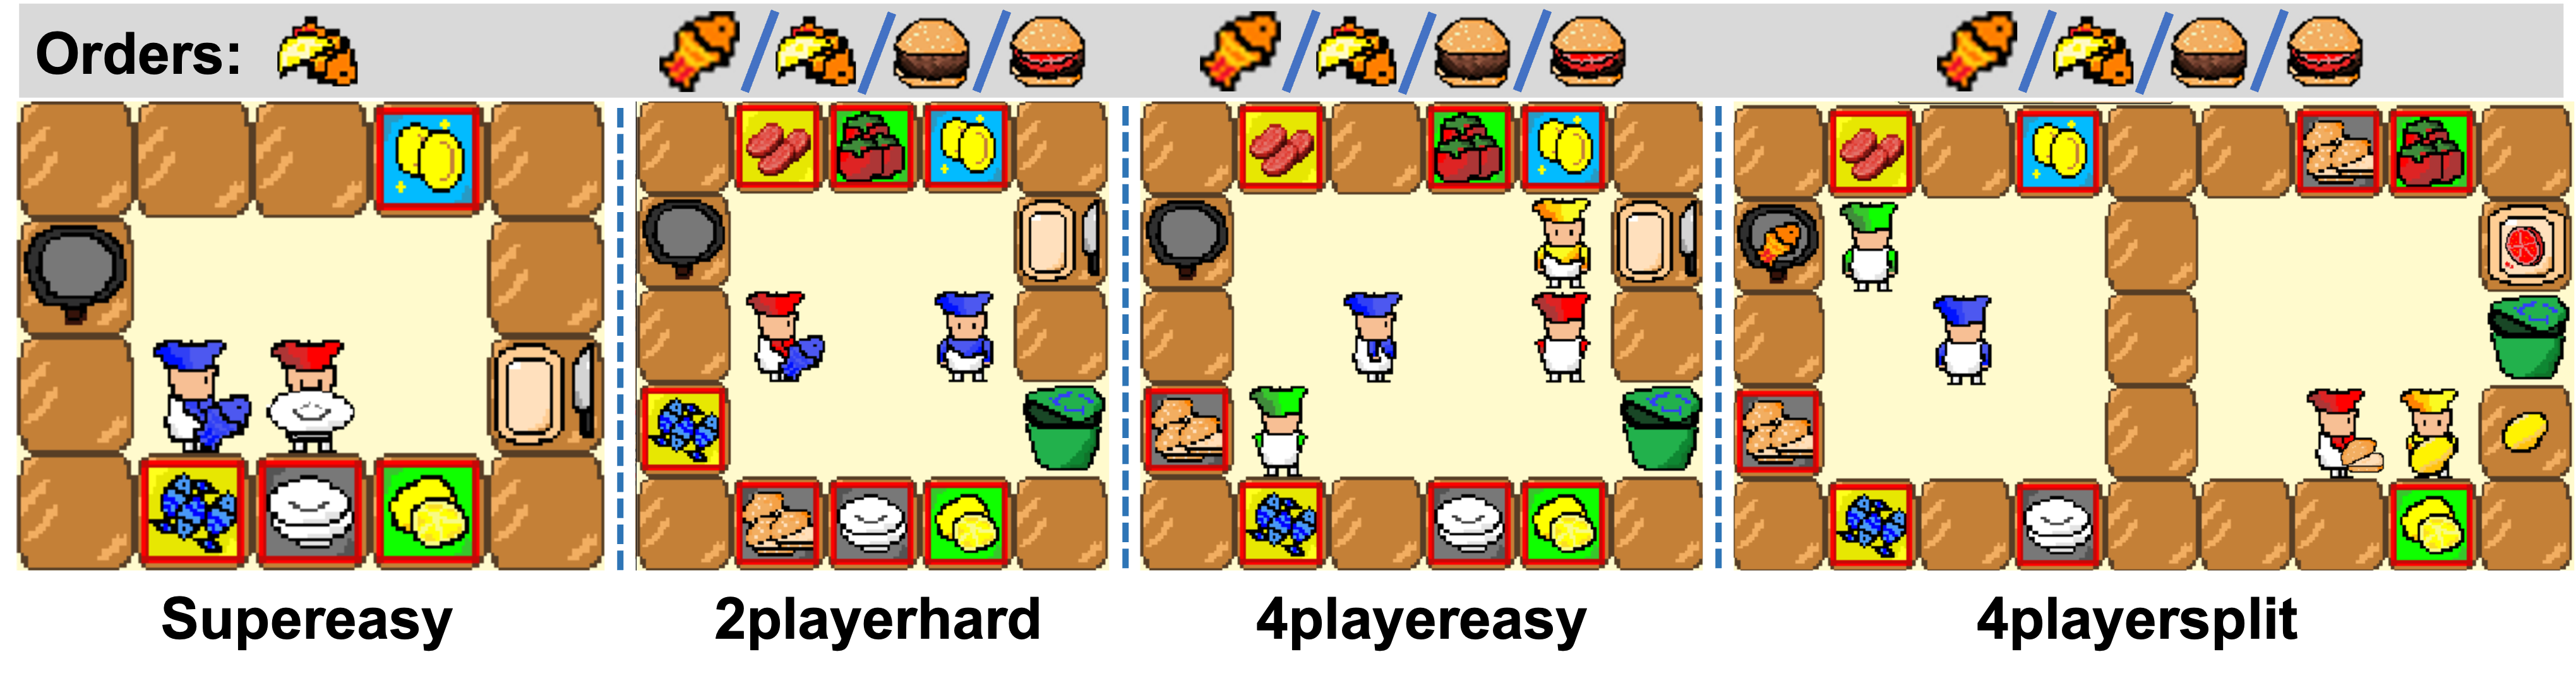
\includegraphics[width=\linewidth]{Figures/4layouts.png}
  \caption{Layouts used in our experiments. From left to right, the difficulty gradually increases. The layout \textit{4playereasy} and \textit{4playersplit} supports four agents playing, and it offers a greater variety of tasks and supports four player interface.}
\label{fig:exp_layouts} 
\end{figure} 
\noindent\textbf{MARL algorithms} \ We use IPPO (independent PPO), VDN and IQL (independent Q-Learning) algorithms. The implementation of these algorithms can be referenced in \cite{papoudakis2020benchmarking}. Hyperparameters can be found in Appendix \ref{appendix:hyper}. \\
\noindent\textbf{Training} \ In each layout, we train MARL agents for 2e7 steps and record average returns over 5 random seeds (Figure \ref{fig:training_curves}). From the training curves we can see that on-policy and off-policy algorithms can converge, but standard deviations seem to be large. In addition, when facing multiple objectives (i.e.,  Figure \ref{fig:training_curves}: b, c, d), the performance of the agents is suboptimal, and it is difficult for them to converge to an ideal reward.

\begin{figure}[H]
    \centering
        \subfloat[Supereasy]{
        \includegraphics[width=0.5\linewidth]{Figures/overcooked2_supereasy_return_mean_True.pdf}}
        \subfloat[2playerhard]{
        \includegraphics[width=0.5\linewidth]{Figures/overcooked2_2playerhard_return_mean_True.pdf}}
        \hfill
        \subfloat[4playereasy]{
        \includegraphics[width=0.5\linewidth]{Figures/overcooked2_4playereasy_return_mean_True.pdf}}
        \subfloat[4playersplit]{
        \includegraphics[width=0.5\linewidth]{Figures/overcooked2_4playersplit_return_mean_True.pdf}}  
    \caption{Training curves of MARL algorithms in four game layouts of \textit{ComplexOvercooked}. The shaded areas denote the standard deviation over five random seeds.}
    \label{fig:training_curves}
\end{figure}


\section{Conclusion and Future Directions}
\label{sec:dis}
\textbf{Conclusion} \ We have introduced an open-source RL environment \textit{ComplexOvercooked}. It is an easily configurable, expandable multi-agent environment, supporting up to four agents in cooperation. It boasts a user-friendly gaming interface and clear underlying game logic and can serve as a benchmark in the field of multi-agent collaboration. We then conducted experiments to validate the environment's usability by using baseline algorithms of MARL. We provide three types of interfaces (i.e., RL agents, humans, and LLM) to control the players, which provide convenience for some valuable future research directions.
\\
\textbf{Future Directions} \ A possible research direction is \textit{human-machine collaboration}. In this multi-task environment, due to the complexity of tasks, it is difficult for a single agent to be competent. Moreover, the workflow for completing tasks is variable. Human players may show behavioral preferences to complete tasks. Training cooperative agents to understand human intentions and to align with human values \cite{yuan2022situ} is worth researching. In fact, Overcooked game greatly necessitates dialogue and communication between players. Due to the urgency of time and orders, partners often need to communicate with each other to achieve better cooperation. Therefore, \textit{collaboration driven by LLMs} is a promising research direction\cite{wen2022multi,zhang2023proagent,zhu2023madiff},. Assisting reinforcement learning algorithms with LLMs could potentially accelerate their convergence. In a dynamic-objective system, \textit{task decomposition and subtask allocation} are also worth studying \cite{yang2022ldsa,iqbal2022alma}. We provide several well-defined tasks in the \textit{ComplexOvercooked}, and subsequent research can focus on enhancing the capabilities of agents in dynamic-objective scenarios.

\bibliographystyle{named}
\bibliography{ref}

\newpage 
\clearpage
\appendix
\section{Hyperparameters of MARL agents}\label{appendix:hyper}
In our experiments, we benchmarks the ippo, vdn and iql MARL algorithms. The specific hyperparameters of PPO and Q-learning are shown in Table \ref{tab:ippo_hyper} and Table \ref{tab:qlearning_hyper}, respectively. Apart from the hyperparameters in the table, we set common hyperparameters of ippo, vdn and iql with an initial learning rate of 1e-3, a reward shaping horizons of half the total timesteps, hidden dim of 64, 128, 256, 256 for the envs \textit{supereasy}, \textit{2playerhard}, \textit{4playereasy}, \textit{4playersplit} respectively. In addition, we set learning rate decay and use a RNN agent in both Q network and PPO policy network. 
\begin{table}[htb]
\centering
\caption{PPO hyperparameters. }
\label{tab:ippo_hyper}
\setlength{\tabcolsep}{3.5mm}
\begin{tabular}{lc}
\toprule
\textbf{Parameter} & \textbf{Value} \\
\midrule
Entropy coefficient        & 0.01         \\
n rollout threads                & 10        \\
Clipping                  & 0.1       \\
PPO epochs                & 8 \\
\bottomrule
\end{tabular}
\end{table}

\begin{table}[htb]
\centering
\caption{Q-learning hyperparameters. }
\label{tab:qlearning_hyper}
\setlength{\tabcolsep}{3.5mm}
\begin{tabular}{lc}
\toprule
\textbf{Parameter} & \textbf{Value} \\
\midrule
Replay buffer size       & 5000         \\
Epsilon start                   & 1        \\
Epsilon finish                     & 0.1        \\
Epsilon anneal time                & 5e6        \\
Target update interval                  & 100       \\
\bottomrule
\end{tabular}
\end{table}









\end{document}
